\documentclass[a4paper,11pt]{ctexart}

\usepackage[margin=2.35cm]{geometry}
\usepackage{amsmath,amssymb,bm}
\usepackage{booktabs}
\usepackage{graphicx}
\usepackage{enumitem}
\usepackage[hidelinks]{hyperref}

\setlist[enumerate]{itemsep=0.25em,topsep=0.4em}
\setlist[itemize]{itemsep=0.25em,topsep=0.4em}
\setlength{\parskip}{0.35em}
\setlength{\parindent}{2em}

\title{\bfseries 光盘光谱仪讲义\\[0.55em]
\large 准直：把入射角的散布收小}
\author{cd\_spectrum}
\date{2026年10月13日}

\begin{document}
\maketitle
\thispagestyle{empty}
\begin{center}
\parbox{0.92\textwidth}{\footnotesize
本讲只处理一件事：进入光盘之前，光束应当有多平行，才能让钠双线的间隔不被入射角的散布吃掉。
全光路画在单独的图里，讲义第~\ref{sec:layout}~节引用它。
数值都以 DVD 的一级衍射、李特罗角附近为准，换盘或换级次时把公式重新代一遍。}
\end{center}
\vspace{0.6em}
\tableofcontents
\vspace{0.8em}

\section{准直要收的是入射角}
\label{sec:why}

光盘上被照亮的那一段，每条轨道都要看到同一个入射角。入射角一旦随位置或随狭缝上的点变化，同一种波长就会落到一段方向上，焦平面上的一条线就变成一条带。

钠双线是后面用来验收的尺度。低压钠灯的两条线在
\[
\lambda_2=588.995\,\mathrm{nm},\qquad \lambda_1=589.592\,\mathrm{nm},
\]
间隔
\[
\Delta\lambda_{\mathrm{Na}}=0.597\,\mathrm{nm}\approx 0.60\,\mathrm{nm}.
\]
要把它们分成两个峰、中间留出一个谷，单条谱线的半高宽需要明显小于这个间隔。本讲把设计目标放在 \(0.2\,\mathrm{nm}\) 附近：狭缝贡献大约 \(0.17\,\mathrm{nm}\)，准直残差再控制在 \(0.1\,\mathrm{nm}\) 以下。高压钠灯和食盐火焰的黄线本身就宽，不能用来做这件验收。

反射光栅的方程写成
\begin{equation}
\label{eq:grating}
m\lambda = d\,(\sin\alpha+\sin\beta).
\end{equation}
\(\alpha\) 是入射角，\(\beta\) 是衍射角，都从法线量起，并且取在法线同一侧。\(d\) 是轨道间距，\(m\) 是级次。DVD 取
\[
d=740\,\mathrm{nm},\qquad m=1.
\]

\section{角误差怎样变成波长误差}
\label{sec:angle}

探测器先选定一个方向 \(\beta\)。这个方向上混进来的波长，来自入射角的差别。对\eqref{eq:grating} 在 \(\beta\) 固定时微分，
\begin{equation}
\label{eq:dlambda}
m\,\Delta\lambda = d\cos\alpha\;\Delta\alpha,
\qquad
\Delta\lambda = \frac{d\cos\alpha}{m}\,\Delta\alpha.
\end{equation}
\(\Delta\alpha\) 用弧度。\(d\) 越大，同样的角度误差换成的波长误差越大，所以 CD（\(d=1600\,\mathrm{nm}\)）比 DVD 更吃准直。

把它倒过来，就是准直的指标。若要求角度残差引起的展宽不超过 \(\Delta\lambda_{\mathrm{col}}\)，则
\begin{equation}
\label{eq:target}
\Delta\alpha \le \frac{m\,\Delta\lambda_{\mathrm{col}}}{d\cos\alpha}.
\end{equation}
李特罗角附近 \(\cos\alpha\approx 0.92\)（第~\ref{sec:littrow}~节）。取 \(\Delta\lambda_{\mathrm{col}}=0.10\,\mathrm{nm}\)，
\begin{equation}
\label{eq:number}
\Delta\alpha \le \frac{0.10}{740\times 0.917}
= 1.5\times 10^{-4}\,\mathrm{rad}
\approx 0.0085^\circ
\approx 0.51'.
\end{equation}
这就是「高精度」在这台装置里的含义：全光束的入射角散布，残差部分要收到大约 \(1.5\times 10^{-4}\,\mathrm{rad}\)。狭缝自己还会贡献一项更大的、但是受控的张角，见第~\ref{sec:slit}~节。

衍射方向上的角色散是另一件事。固定 \(\alpha\)，对 \(\beta\) 微分，
\begin{equation}
\label{eq:dispersion}
\frac{\mathrm{d}\beta}{\mathrm{d}\lambda}
= \frac{m}{d\cos\beta}.
\end{equation}
钠双线在李特罗角附近的角距只有
\begin{equation}
\Delta\beta
= \frac{0.597}{740\times 0.917}
= 8.8\times 10^{-4}\,\mathrm{rad}
\approx 0.050^\circ.
\end{equation}
图上如果把双线画成明显的两个方向，那是夸大，不是实物的夹角。

\section{狭缝放在透镜的焦平面上}
\label{sec:slit}

一块焦距 \(f\) 的透镜，物在焦平面上时，出射光束平行。狭缝宽 \(w\)，放在这块透镜的焦平面上，狭缝两端发出的主光线夹角是
\begin{equation}
\label{eq:slitangle}
\Delta\alpha_w = \frac{w}{f}.
\end{equation}
代回\eqref{eq:dlambda}，狭缝单独造成的谱线宽度是
\begin{equation}
\label{eq:slitlambda}
\Delta\lambda_w = \frac{d\cos\alpha}{m}\,\frac{w}{f}.
\end{equation}
同一块透镜把返回的衍射光再会聚到焦平面时，线色散为
\begin{equation}
\label{eq:linear}
\frac{\mathrm{d}x}{\mathrm{d}\lambda}
= f\,\frac{m}{d\cos\beta}.
\end{equation}
李特罗条件下 \(\alpha\approx\beta\)，狭缝像的横向放大率接近 \(1\)，所以 \(\Delta\lambda_w\) 也等于缝宽除以线色散。

取 \(f=200\,\mathrm{mm}\)、\(w=50\,\mu\mathrm{m}=0.050\,\mathrm{mm}\)：
\begin{align}
\Delta\alpha_w &= \frac{0.050}{200} = 2.5\times 10^{-4}\,\mathrm{rad}, \\[0.3em]
\Delta\lambda_w &= 740\times 0.917\times 2.5\times 10^{-4}
= 0.17\,\mathrm{nm}.
\end{align}
\(0.17\,\mathrm{nm}\) 是 \(0.60\,\mathrm{nm}\) 的四分之一强，双线中间可以出现谷。线色散
\[
\frac{\mathrm{d}x}{\mathrm{d}\lambda}
= 200\times\frac{1}{740\times 0.917}
= 0.295\,\mathrm{mm\,nm^{-1}},
\]
双线在焦平面上分开
\[
\Delta x = 0.295\times 0.597 = 0.18\,\mathrm{mm}.
\]
卸掉镜头的 CMOS 放在这个焦平面上，像素尺寸是微米量级，采样是够的。限制来自缝宽、离焦和光盘，不来自像素太少。

焦距取长，同样的缝宽对应更小的 \(\Delta\alpha_w\)。\(f=200\,\mathrm{mm}\) 配 \(50\,\mu\mathrm{m}\) 的刀片狭缝，是实验室里做得到的组合。若改用 \(f=50\,\mathrm{mm}\) 的镜头，要维持同样的 \(\Delta\lambda_w\)，缝宽得收到 \(12\,\mu\mathrm{m}\) 左右，通光量和缝的平直度都会变紧。

透镜要收到大约 \(D=10\,\mathrm{mm}\) 的通光口径，相对孔径大约 \(f/20\)。廉价消色差双胶合在这个口径下，剩余像差比 \(0.1\,\mathrm{nm}\) 的指标小。口径再放大，球差和场曲先变坏，同时照亮的轨道更长，弯曲轨道会把谱线拉弯。

只检验钠双线时，透镜对 \(589\,\mathrm{nm}\) 调焦即可。若整段可见光都要同样平行，消色差双胶合仍可用；凹面反射镜没有色差，焦距同样取 \(200\,\mathrm{mm}\) 量级，口径同样收到 \(f/10\) 以下。

\subsection{离焦还剩多少张角}

狭缝沿光轴偏离焦平面 \(\delta z\) 时，出射光束不再平行。光束直径为 \(D\)，边缘相对中心的偏角约为 \(D\,|\delta z|/(2f^2)\)，两边合起来的全张角约为
\begin{equation}
\label{eq:defocus}
\Delta\alpha_{\mathrm{def}} \approx \frac{D\,|\delta z|}{f^2}.
\end{equation}
让这一项小于狭缝张角 \(w/f\)，
\begin{equation}
\label{eq:tolerance}
|\delta z| < \frac{w f}{D}.
\end{equation}
代入 \(w=0.050\,\mathrm{mm}\)、\(f=200\,\mathrm{mm}\)、\(D=10\,\mathrm{mm}\)，
\[
|\delta z| < 1.0\,\mathrm{mm}.
\]
自准直时把狭缝放在焦平面前后 \(1\,\mathrm{mm}\) 以内，就满足这个设计。若还要把离焦展宽压到 \(0.10\,\mathrm{nm}\) 以下，对应的 \(\Delta\alpha_{\mathrm{def}}\) 约为 \(1.5\times 10^{-4}\,\mathrm{rad}\)，
\[
|\delta z|
< \frac{1.5\times 10^{-4}\times 200^2}{10}
= 0.6\,\mathrm{mm}.
\]
调节时以 \(0.6\,\mathrm{mm}\) 为目标，\(1\,\mathrm{mm}\) 作为还可以接受的上限。

\section{没有准直透镜时的下限}
\label{sec:nolens}

狭缝到光盘的距离若是 \(L\)，中间没有透镜，照亮宽度 \(W\) 的两端入射角大约差 \(W/L\)。由\eqref{eq:dlambda}，
\begin{equation}
\Delta\lambda_g = \frac{d\cos\alpha}{m}\,\frac{W}{L}.
\end{equation}
照亮的轨道数 \(N=W/d\)，光栅衍射极限给出的宽度是
\begin{equation}
\Delta\lambda_d = \frac{\lambda}{m N} = \frac{\lambda d}{m W}.
\end{equation}
\(W\) 加大，衍射极限变好，几何张角变差。令两项相等，
\begin{equation}
\label{eq:wopt}
W = \sqrt{\frac{\lambda L}{\cos\alpha}},
\qquad
\Delta\lambda_{\min}
= \frac{d}{m}\sqrt{\frac{\lambda\cos\alpha}{L}}.
\end{equation}
这是量级估计：真正的线宽还要叠上缝宽、保护层里的散射和轨道弯曲。

对 DVD，取 \(\lambda=589\,\mathrm{nm}\)、\(\cos\alpha\approx 1\)、\(L=1\,\mathrm{m}\)，
\[
\Delta\lambda_{\min}
= 740\times\sqrt{\frac{589}{10^{9}}}
= 0.57\,\mathrm{nm},
\qquad
W\approx 0.77\,\mathrm{mm}.
\]
\(0.57\,\mathrm{nm}\) 已经和双线间隔一样大。一米长的自由传播，刚好摸到钠双线，缝、保护层和离焦都没有余量。距离缩到 \(20\,\mathrm{cm}\) 时，这个下限大约变成 \(1.3\,\mathrm{nm}\)，双线会并成一条。

准直透镜改变的是这件事：平行光的入射角不再由 \(W/L\) 决定。\(W\) 可以收到几毫米到大约 \(10\,\mathrm{mm}\)，轨道数足够，\(R=mN\) 远高于 \(10^3\)；波长宽度改由\eqref{eq:slitlambda} 和\eqref{eq:defocus} 决定。

\section{李特罗光路}
\label{sec:littrow}

李特罗条件是衍射光大致沿入射光的反方向回去，即 \(\beta=\alpha\)。代入\eqref{eq:grating}，
\begin{equation}
\label{eq:littrow}
m\lambda = 2d\sin\alpha,
\qquad
\alpha_L = \arcsin\frac{m\lambda}{2d}.
\end{equation}
对双线的平均波长 \(\lambda=589.3\,\mathrm{nm}\)、\(m=1\)、\(d=740\,\mathrm{nm}\)，
\begin{equation}
\sin\alpha_L = \frac{589.3}{2\times 740} = 0.398,
\qquad
\alpha_L = 23.4^\circ,
\qquad
\cos\alpha_L = 0.917.
\end{equation}
光盘法线相对入射光束偏过 \(23.4^\circ\)，光栅面相对垂直位置也偏过这个角度。\(589\,\mathrm{nm}\) 附近的一级光返回透镜，再会聚到焦平面上、狭缝旁边。零级是镜面反射，相对法线的出射角等于入射角，不回到这块透镜里。

因此准直和探测是同一块透镜的两次使用：
\begin{itemize}
\item 去程：狭缝在焦平面上，透镜把光收成平行光，照到光盘上被掩模留出的窄带。
\item 回程：不同波长以略有差别的方向返回，透镜把每一个方向会聚成狭缝的一个像。像的位置由\eqref{eq:linear} 决定。
\end{itemize}
CMOS 放在这个焦平面上，镜头卸掉。曝光、增益和白平衡全部手动并锁死，能存原始数据就存原始数据。先拍一张挡住狭缝的暗场。波长只从已知谱线的像素位置标定，峰的高度在辐射响应校正之前只表示这台相机的读数。

轨道的局部方向要和狭缝平行，掩模以外的盘面遮住。照亮整张光盘时，圆弧轨道的方向在变，谱线会弯。

\section{调节步骤}
\label{sec:align}

平行光管先单独调，光盘先不装。

\begin{enumerate}
\item \textbf{自准直。} 照亮狭缝，在出射光束中放一块平面镜，让光返回。沿光轴移动狭缝，直到返回的缝像与狭缝重合、两边同时清楚。光走了来回，离焦看得更明显。
\item \textbf{刀口。} 在狭缝平面用刀片切割返回光束。准直到位时，整个光斑一起变暗。暗影从一侧扫到另一侧，说明狭缝还在焦前或焦后。
\item \textbf{远场。} 拿走平面镜，让光束射到数米外的墙上。全张角 \(1.5\times 10^{-4}\,\mathrm{rad}\) 时，\(5\,\mathrm{m}\) 处光斑只比近处胀大约 \(0.75\,\mathrm{mm}\)。胀得明显更多，就回到第 1 步。
\end{enumerate}

光盘按 \(23.4^\circ\) 装上之后，只改缝宽做一次检查。谱线还在变窄，就继续收缝；不再变窄，而双线仍然连在一起，就查离焦、掩模和轨道是否平直。验收光源用低压钠灯。

实验室里的分光计平行光管就是「狭缝 + 消色差物镜」，并且通常已经按自准直调过。把它当作本节的透镜，光盘放在载物台上，是同一套原理。

\section{一套可以开工的数值}
\label{sec:numbers}

\begin{table}[htbp]
\centering
\caption{DVD、一级、钠黄光附近的设计点}
\label{tab:design}
\begin{tabular}{ll}
\toprule
量 & 取值 \\
\midrule
轨道间距 \(d\) & \(740\,\mathrm{nm}\) \\
级次 \(m\) & \(1\) \\
设计波长 & \(589.3\,\mathrm{nm}\) \\
李特罗角 \(\alpha_L\) & \(23.4^\circ\) \\
透镜焦距 \(f\) & \(200\,\mathrm{mm}\) \\
通光口径 \(D\) & \(10\,\mathrm{mm}\) \\
狭缝宽度 \(w\) & \(50\,\mu\mathrm{m}\) \\
缝的张角 \(w/f\) & \(2.5\times 10^{-4}\,\mathrm{rad}\) \\
缝引起的 \(\Delta\lambda_w\) & \(0.17\,\mathrm{nm}\) \\
准直残差目标 \(\Delta\lambda_{\mathrm{col}}\) & \(\le 0.10\,\mathrm{nm}\) \\
对应的残差张角 & \(\le 1.5\times 10^{-4}\,\mathrm{rad}\) \\
离焦容许 & \(0.6\,\mathrm{mm}\)（目标），\(1\,\mathrm{mm}\)（上限） \\
线色散 & \(0.295\,\mathrm{mm\,nm^{-1}}\) \\
双线在焦平面上的间隔 & \(0.18\,\mathrm{mm}\) \\
双线的实际角距 & \(0.050^\circ\) \\
\bottomrule
\end{tabular}
\end{table}

换用 CD 时，\(d=1600\,\mathrm{nm}\)，同一波长的李特罗角变为
\[
\alpha_L = \arcsin\frac{589.3}{3200} = 10.6^\circ.
\]
\eqref{eq:slitlambda} 里的 \(d\cos\alpha\) 大约增大到 \(2.3\) 倍，同样的缝和焦距给出 \(\Delta\lambda_w\approx 0.39\,\mathrm{nm}\)。双线仍有可能分开，余量小很多。CD 的保护层也更厚。第一台高分辨率装置用 DVD。

\section{全光路}
\label{sec:layout}

图~\ref{fig:layout} 是按本节光路画的示意图，单独的文件是 \texttt{光路图/全光路.pdf}。看图时抓住四件事。

\begin{enumerate}
\item 低压钠灯只照亮焦平面上的狭缝。狭缝到透镜的距离是 \(f\)。
\item 透镜之后，射向光盘的是一束平行光。光盘法线相对这束光偏过 \(\alpha=23.4^\circ\)。
\item \(589.0\,\mathrm{nm}\) 和 \(589.6\,\mathrm{nm}\) 沿两个略有差别的方向返回，再次经过同一块透镜，会聚到焦平面上的两个点。探测器是卸掉镜头的 CMOS，就放在这两个点所在的平面上。
\item 零级沿镜面反射方向离开，不进入透镜。
\end{enumerate}

\begin{figure}[htbp]
\centering
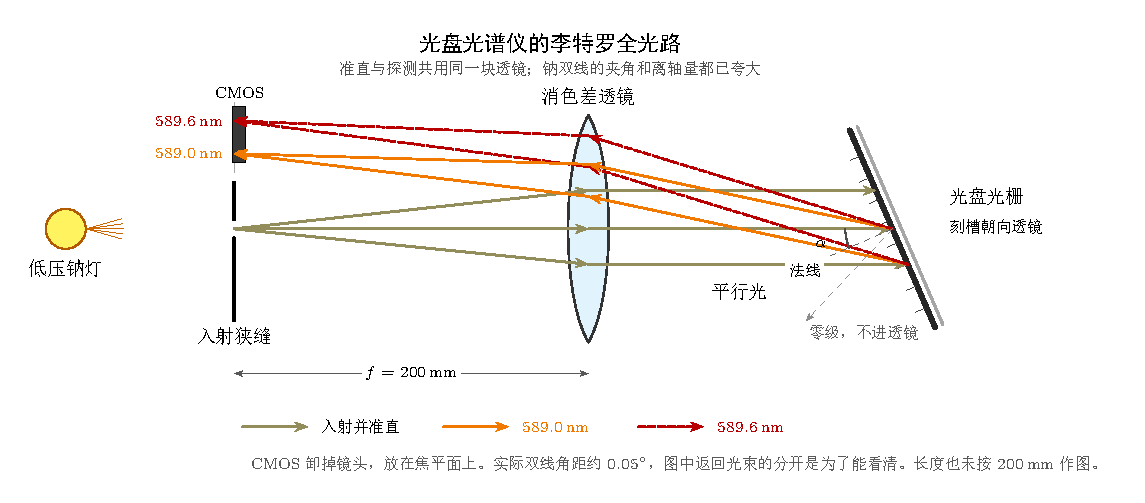
\includegraphics[width=\textwidth]{../../光路图/全光路.pdf}
\caption{李特罗全光路。返回光束的夹角和离轴量都画大了：钠双线的实际角距约 \(0.05^\circ\)，在 \(f=200\,\mathrm{mm}\) 的焦平面上只分开 \(0.18\,\mathrm{mm}\)。图中的长度也没有按 \(200\,\mathrm{mm}\) 缩放。}
\label{fig:layout}
\end{figure}

\section{小结}

入射角的散布按 \(\Delta\lambda=(d\cos\alpha/m)\,\Delta\alpha\) 变成谱线宽度。DVD 在李特罗角附近，要把这项残差压到 \(0.10\,\mathrm{nm}\)，全光束的角度残差大约是 \(1.5\times 10^{-4}\,\mathrm{rad}\)。

做法是把 \(50\,\mu\mathrm{m}\) 的狭缝放在 \(f=200\,\mathrm{mm}\) 消色差透镜的焦平面上，通光口径收到约 \(10\,\mathrm{mm}\)，离焦控制在 \(1\,\mathrm{mm}\) 以内，并用平面镜返回的缝像来调。光盘放在 \(23.4^\circ\)。同一块透镜把一级衍射送回焦平面，卸掉镜头的 CMOS 在那里记录。缝宽单独留下约 \(0.17\,\mathrm{nm}\)，双线间隔 \(0.60\,\mathrm{nm}\)，中间有地方出现谷。

没有这块透镜时，照亮宽度和入射角散布绑在一起。一米的距离刚刚摸到 \(0.6\,\mathrm{nm}\)，没有余量。

\end{document}
